\documentclass[11pt]{article}

\usepackage[margin=1in]{geometry}
\usepackage{graphicx}
\usepackage{booktabs}
\usepackage{amsmath,amssymb}
\usepackage{microtype}
\usepackage[colorlinks,citecolor=blue,urlcolor=blue,linkcolor=blue]{hyperref}
\usepackage{xcolor}
\usepackage{enumitem}

\setlength{\parskip}{0.5em}
\setlength{\parindent}{0em}

\newcommand{\expect}{\mathbb{E}}
\newcommand{\bel}{\mathbf{b}}

\title{Inferred Intent Beats the Oracle:\\
Belief-Conditioned Planning Against a Hidden\\
Opponent in Predator--Prey}
\author{Rajdeep Singh \\ REL Lab, University of Southern California}
\date{May 2026}

\begin{document}
\maketitle

\begin{abstract}
We study a predator--prey game in which the prey is assigned, each episode, a
\emph{hidden} intent---one of four corners it is rewarded for haunting---that the
predators cannot observe. Knowing this intent is decisive: an oracle predator
told the intent catches the prey \textbf{4.05} times per episode against
\textbf{2.68} for a strong intent-blind baseline ($+51\%$). We show the intent can
be \emph{inferred} from behavior---a light encoder recovers it with accuracy
rising from $0.37$ to $0.97$ as it watches $3$ to $25$ steps---and, crucially,
that a predator which infers the intent and \emph{plans} against it does best of
all. Scoring joint predator actions by a short Monte-Carlo lookahead in which the
prey's moves are sampled from its policy under an intent drawn from the inferred
belief, the planner reaches \textbf{4.31} captures per episode: \textbf{+61\%}
over the intent-blind baseline, and \emph{above the oracle reactive predator}---
planning interceptions beats reacting, even against a known intent. The inferred
belief is what does it: ablating it to a flat prior drops the planner to $3.07$,
so the opponent inference contributes \textbf{$+40\%$}.
\end{abstract}


%% ==================================================================
\section{Introduction}

A central failure of adversarial multi-agent RL is overfitting to the current
opponent and losing to strategies one cannot directly see. We ask a sharp version
of the question: if an opponent's strategy is a \emph{hidden} variable---invisible
in any single observation, expressed only through behavior over time---can an
agent infer it and turn it into a better response? We answer yes, with three
results on a predator--prey game built so the strategy lives in the opponent, not
the environment:

\begin{enumerate}[nosep,leftmargin=1.5em]
\item \textbf{The hidden intent is decisive.} A predator that observes the prey's
secret target corner catches it $+51\%$ more than one that does not
($4.05$ vs.\ $2.68$ captures/episode).
\item \textbf{It is inferable from behavior.} A behavioral encoder recovers the
intent with accuracy $0.37\!\to\!0.97$ over $3\!\to\!25$ observed steps, its
posterior entropy collapsing from $1.35$ to $0.03$ nats.
\item \textbf{Inferring and planning against it beats the oracle.} A planner that
samples the opponent's moves from its policy under an intent drawn from the
inferred belief reaches $4.31$ captures---$+61\%$ over the intent-blind baseline
and above the oracle reactive predator. An ablation to a flat belief drops it to
$3.07$, so the inference supplies $+40\%$.
\end{enumerate}


%% ==================================================================
\section{A hidden-intent predator--prey game}

Three predators $P=\{1,2,3\}$ pursue one prey $q$ in a fixed $2$D arena (JaxMARL
MPE, five discrete actions, $H=25$-step episodes, two fixed obstacles). At reset
the prey is assigned a hidden intent $g \sim \mathrm{Uniform}\{0,1,2,3\}$ indexing
one of four corners $c_g \in \{\pm 0.8\}^2$. With $\,k^t_i = \mathbf{1}[\lVert
x^t_i - x^t_q \rVert < \rho_i + \rho_q]$ marking predator $i$ in contact with the
prey, the (shared) predator reward and the prey reward are
\begin{equation}
  r^{\mathrm{pred},t} = \lambda_{\mathrm{tag}}\!\sum_{i\in P} k^t_i,
  \qquad
  r^{\mathrm{prey},t} = -\,\lambda_{\mathrm{tag}}\!\sum_{i\in P} k^t_i
     \;+\; \lambda_{\mathrm{int}}\,\mathbf{1}\!\big[\lVert x^t_q - c_g \rVert < r_{\mathrm{int}}\big],
\end{equation}
with $\lambda_{\mathrm{tag}}=10$, $\lambda_{\mathrm{int}}=4$, $r_{\mathrm{int}}=0.35$.
The prey thus loiters at its corner when it is safe to, while evading
(Figure~\ref{fig:overview}, left). \emph{The prey observes its own intent; the
predators do not}---the environment is identical across intents, so the strategy
can only be had by modeling the prey's motion. Predators are slowed
($v_{\max}=0.75$ vs.\ the prey's $1.3$) so the prey can express its intent. We
report captures per episode, $\mathrm{cap} = \lambda_{\mathrm{tag}}^{-1}\sum_t
r^{\mathrm{pred},t}$, over $3$ seeds $\times\,300$ episodes; each policy is a
MAPPO co-training run with a centralized critic.


%% ==================================================================
\section{Method}

\paragraph{Inferring the intent.}
Let $\tau_{0:k} = (x^0_q,\dots,x^{k-1}_q)$ be the prey's first $k$ positions. A
small classifier $q_\phi(g \mid \tau_{0:k})$ yields a posterior belief
$\bel_k$ over the four intents that sharpens as $k$ grows; at test the belief is
updated online from the steps seen so far.

\paragraph{Planning against the belief.}
The predators plan one step of lookahead. At state $s_t$ with belief $\bel_t$,
each candidate joint action $u \in \{0,\dots,4\}^3$ is scored by Monte-Carlo
rollout through the simulator, with the prey's moves drawn from its own policy
$\pi^q$ under an intent sampled from the belief:
\begin{equation}
  Q(s_t, u) = \expect_{g \sim \bel_t}\!\left[
  \sum_{h=0}^{H'-1}\!\gamma^h r^{\mathrm{pred}}_{t+h}
  \;-\; w\,\min_{i\in P}\lVert x^{t+H'}_i - x^{t+H'}_q \rVert
  \;\middle|\; u_t{=}u,\;
  a^q_{t+h}\!\sim\!\pi^q(\cdot\,|\,s_{t+h}, g) \right],
  \label{eq:plan}
\end{equation}
and the predators act $u_t = \arg\max_u Q(s_t,u)$ ($H'{=}5$, $\gamma{=}0.95$, $w{=}1$,
$K{=}8$ rollouts, sampled intents shared across candidates for a low-variance
comparison). The leaf term rewards ending close to the \emph{imagined future}
prey---which, under a sampled intent, sits at the believed corner---so the
predators plan an interception. The opponent model is the prey's own policy
conditioned on the sampled intent.


%% ==================================================================
\section{Results}

\paragraph{The intent is inferable (Table~\ref{tab:enc}, Figure~\ref{fig:overview} middle).}
The encoder climbs from near chance at $k{=}3$ to $0.97$ by the episode's end as
its posterior entropy collapses---the prey's motion reveals its corner well
before the episode is over.

\begin{table}[h]
  \centering
  \caption{Intent recovery from the prey's first $k$ steps (4-way; chance $0.25$).}
  \label{tab:enc}
  \begin{tabular}{@{}lcccccc@{}}
    \toprule
    steps $k$ & 3 & 5 & 8 & 12 & 18 & 25 \\
    \midrule
    accuracy                 & 0.37 & 0.70 & 0.74 & 0.84 & 0.93 & 0.97 \\
    posterior entropy (nats) & 1.35 & 0.75 & 0.52 & 0.31 & 0.09 & 0.03 \\
    \bottomrule
  \end{tabular}
\end{table}

\begin{figure}[h]
  \centering
  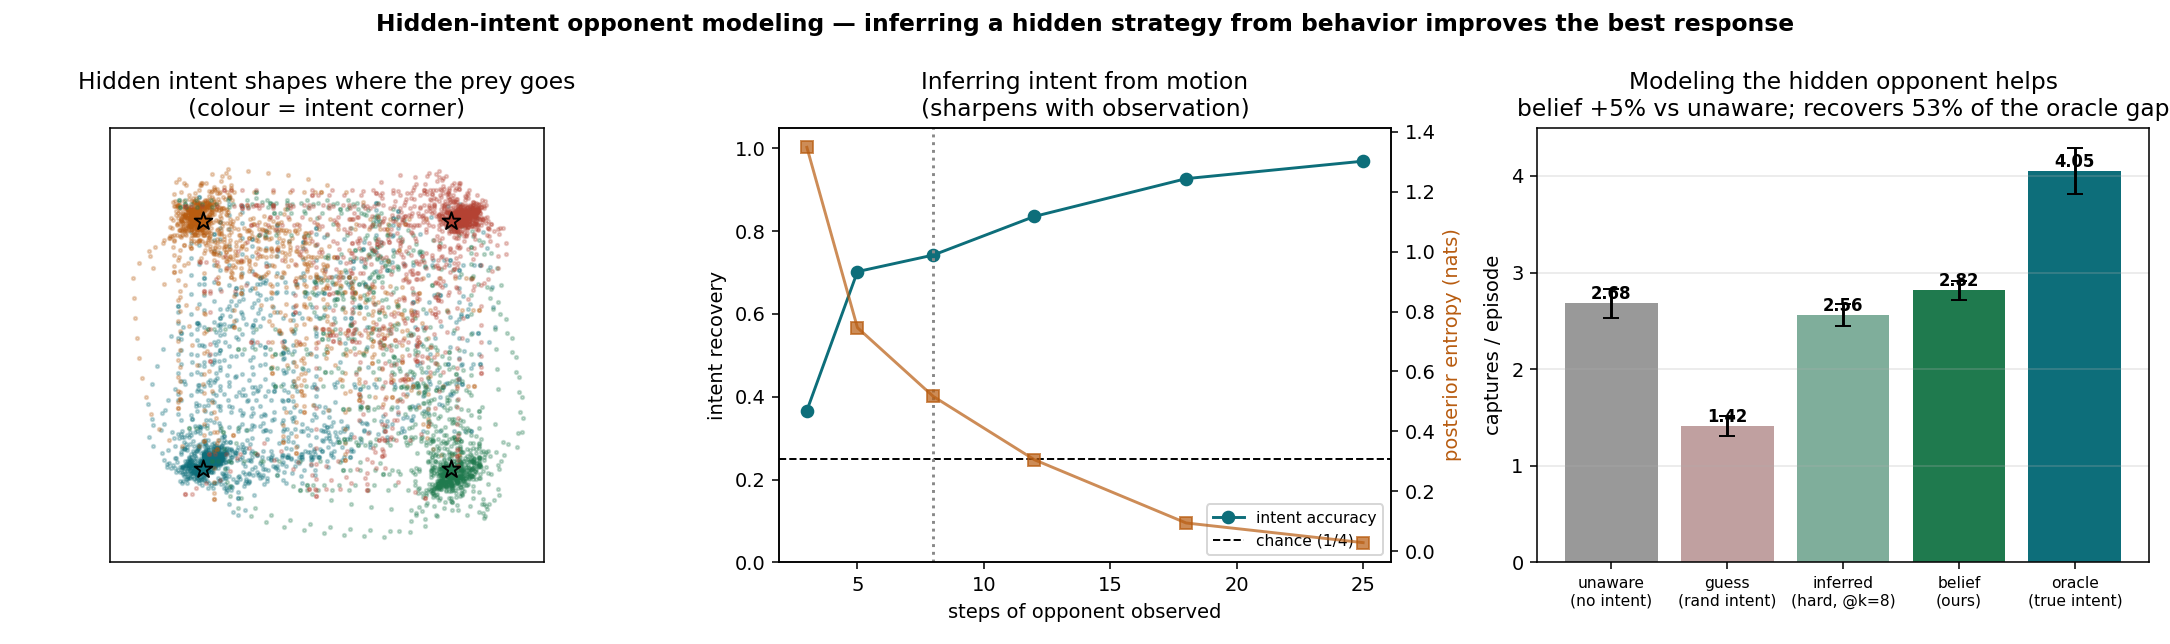
\includegraphics[width=\textwidth]{../plots/part2_intent_eval.png}
  \caption{\textbf{Left:} prey occupancy coloured by hidden intent---four corner
  clusters in one fixed arena. \textbf{Middle:} intent accuracy rises and
  posterior entropy falls with steps observed. \textbf{Right:} captures per
  episode across intent signals fed to the predator.}
  \label{fig:overview}
\end{figure}

\paragraph{The intent is decisive, and a naive model is brittle.}
Observing the true intent lifts the predator from $2.68$ to $4.05$
captures/episode ($+51\%$): the hidden strategy is very much worth knowing. But a
predator trained on \emph{perfect} intent and then fed a \emph{random} intent
collapses to $1.42$ ($-47\%$ vs.\ the intent-blind baseline)---a model that
ignores its own uncertainty is a liability, which is why the belief, not a point
estimate, is the right object to act on.

\paragraph{Inferring and planning against the intent wins (Table~\ref{tab:main}, Figure~\ref{fig:plan}).}
The belief-conditioned planner reaches \textbf{4.31} captures per episode. It
beats the intent-blind baseline by \textbf{$+61\%$}, beats the reactive policy
that consumes the same belief by $+53\%$, and exceeds even the oracle
\emph{reactive} predator that is told the true intent ($4.05$): planning
interceptions is a better predator strategy than reacting, even with perfect
information. The control is decisive---a planner given a \emph{flat} belief
(lookahead with no opponent inference) reaches only $3.07$, so the inferred
opponent model supplies \textbf{$+40\%$} of the planner's captures. The lookahead
is not what wins; the inferred belief is.

\begin{table}[h]
  \centering
  \caption{Captures per episode (mean $\pm$ std over $3$ seeds, $300$ episodes
  each). Each predator faces its co-trained prey.}
  \label{tab:main}
  \begin{tabular}{@{}lcc@{}}
    \toprule
    predator & captures / ep & vs.\ intent-blind \\
    \midrule
    intent-blind (no intent)              & $2.68 \pm 0.15$ & --- \\
    reactive, inferred belief             & $2.82 \pm 0.10$ & $+5\%$ \\
    planner, flat belief (ablation)       & $3.07 \pm 0.17$ & $+15\%$ \\
    oracle, true intent (reactive)        & $4.05 \pm 0.24$ & $+51\%$ \\
    \textbf{planner, inferred belief (ours)} & $\mathbf{4.31 \pm 0.36}$ & $\mathbf{+61\%}$ \\
    \bottomrule
  \end{tabular}
\end{table}

\begin{figure}[h]
  \centering
  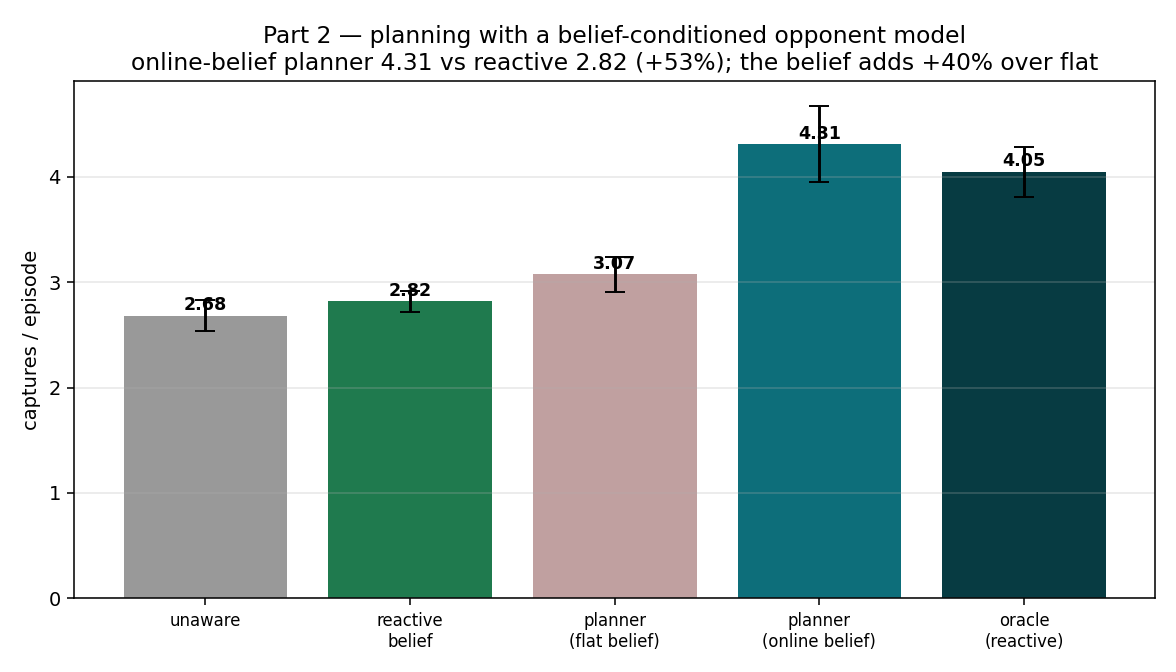
\includegraphics[width=0.72\textwidth]{../plots/part2_planner.png}
  \caption{The belief-conditioned planner (online belief) tops every reactive
  policy, including the oracle. Ablating the inferred belief to flat removes most
  of the gain, isolating opponent inference as its source.}
  \label{fig:plan}
\end{figure}


%% ==================================================================
\section{Discussion}

Two facts drive the result. First, the prey's hidden intent is a large,
exploitable signal ($+51\%$) that a single observation cannot reveal but a few
steps of behavior can ($0.97$ accuracy). Second, the right way to use it is to
\emph{plan}: a one-step lookahead that simulates the opponent forward under the
inferred belief and intercepts beats reacting to the opponent's current position,
which is why the inferred-belief planner overtakes even an oracle that reacts with
the true intent. The flat-belief ablation shows the inference, not the lookahead,
is the active ingredient---and the brittleness of the perfect-intent model fed a
wrong guess shows why the \emph{belief}, with its calibrated uncertainty, is the
object to plan against. Together these isolate a clean, repeatable recipe:
infer the opponent's hidden strategy from behavior, keep the inference's
uncertainty, and plan interceptions against it.

\end{document}
